\section{Context of the thesis}
\subsection{The reproducibility crisis}
\label{sec:reproducibility_crisis}
Even though thousands of papers are published every year about different aspects of the brain, our understanding of this complex organ has not scaled in proportion. A large part of the reason has been attributed to what is known as the reproducibility crisis~\citep{ioannidis2005most, simmons2011false, button2013power}. %Replication is closely related to the concept of reproducibility which refers to the idea that an experiment produces the same result when performed again under the same conditions. Replication is a stronger condition as it requires similar results or identical conclusion even if there are some minor variations in the experimental procedures. 
Progress in science rests on reproducible experiments. Reproducibility refers to the fact that the findings of an experiment can be regenerated if the code, data, and related software was provided to an independent . In many fields, however, a large fraction of experiments cannot be reproduced. In psychology, for instance, it was estimated that over half of the papers were not reproducible~\citep{open2015estimating}, and even those which could be reproduced tended to have a weaker effect size compared to the original study. 

The reasons for unreproducible results can be many~\citep{baker20161}, some being: 1) confirmation bias, the tendency to selectively report only experiments that conform to the researcher's pre-existing beliefs, 2) ``p-hacking''~\citep{simmons2011false}, or the tendency to try multiple hypothesis to get a positive result, 3) publication bias or the absence of incentives to publish negative results~\citep{rosenthal1979file}, and 4) pressure to publish. There are now an accepted set of recommendations to counter many of these issues: 1) pre-registering research plans to avoid confirmation bias and even report negative results, 2) correct for multiple comparisons, the most conservative method being the Bonferroni correction~\citep{dunn1961multiple}. 

Brain imaging has its own set of issues which can be linked to reproducibility crisis: 

% vul2009puzzlingly
% yendiki2014spurious

\begin{itemize}[noitemsep,partopsep=0pt]
\item \textbf{Power failure:} This is arguably one of the central issues in the reproducibility crisis today and has received by far the most attention. The statistical power of a study refers to the likelihood of discovering an effect of interest, given the sample size. Small sample sizes translate into underpowered studies which means that the chance of a false discovery is high. In order to discover the effect of interest, the study must be appropriately powered.
\item \textbf{Multiple comparison:} This is essentially a manifestation of ``p hacking'' that is a result of of the large number of voxels or time points in neuroimaging. For instance, in the famous dead salmon study~\citep{bennett2009neural}, a significant effect was found even if none was expected simply because the hypothesis testing (comparisons) were done over each voxel.
\item \textbf{Differences in software versions:} Changing software versions can lead to different results. For instance in the case of Freesurfer software, differences in volume were found in the range of $8.8\% \pm 6.6\%$ was found~\citep{gronenschild2012effects}.
\item \textbf{Complex pipelines:} Neuroimaging pipelines involve a number of choices at each processing stage, and there isn't currently a consensus on how to choose the right pipeline. Often, these methodological choices are not even documented. It is estimated that almost every new study has its own unique pipeline~\citep{Carp2012289}.
\item \textbf{Confounds:} There are several methodological confounds such as head movements~\citep{yendiki2014spurious}, anatomy differences, and changes in breathing rate and depth, which can lead to spurious correlations.
\end{itemize}

In Chapter~\ref{chapter:group_study} of the thesis, we will provide concrete guidelines on how to build processing pipelines for \ac{MEG}/\ac{EEG} data. Our contribution will touch upon the issue of complex pipelines, multiple comparison, and differences in software versions in the context of \ac{MEG}/\ac{EEG}. The issue of power failure can be alleviated through data sharing as I will discuss in the next section.

\subsection{Data sharing}
\label{sec:intro_datasharing}
Power failure is essentially a consequence of small datasets. In today's collaborative and data-driven scientific environment, data sharing is useful not only from the perspective of reproducibility but also to build datasets with large sample sizes. With large datasets, it would be possible to tease apart even subtle effects~\citep{smith2017statistical} that were not possible with smaller datasets. Data sharing is beneficial not just from the perspective of replication but also from an economic perspective. Rather than collect new data for every new hypothesis, researchers can now reuse known data for answering their hypotheses.

The benefits of data sharing can be traced back to Newton and his theory of gravitation~\citep{pointofview2013}. Before Newton had developed his theory, another English astronomer, John Flamsteed had been appointed by the king to observe the stars and produce accurate charts for navigation in the seas. Over a period of 40 years, Flamsteed created a detailed catalogue that tripled the number of entries in the previously used sky atlas. When the great comet of 1680 appeared in the sky twice in close succession, Flamsteed used his data to postulate that it was not two comets but in fact the same comet which first went towards the sun and then turned away from it. Newton initially opposed this theory, but later changed his mind as he gained access to Flamsteed's unpublished catalogue. The comet had indeed turned out to be an important benchmark for Newton's theory of gravitation.

It is hard to imagine in this day and age that a theory as fundamental as the laws of gravitation could have been data driven. Data sharing is fundamental not only to reproducible science, but also it forms the cornerstone for learning stronger models and benchmarking new algorithms. Consequently, in machine learning, recent breakthroughs have been powered by the increase in data sharing and computation. This includes the recent resurgence of deep learning~\citep{deng2009imagenet}, Q learning~\citep{watkins1992q, bellemare2013arcade}, natural language processing for language translation~\citep{halevy2009unreasonable}, speech recognition~\citep{paul1992design}, and even the mixture of experts model~\citep{jacobs1991adaptive} for IBM Watson~\citep{ferrucci2010building}. The maxim, ``more data beats a cleverer algorithm''~\citep{domingos2012few} has held up remarkably well across disciplines and over the ages.

Of course, neuroscientists are beginning to realize the importance of sharing data. In recent times, neural data has started being shared through international consortiums~\citep{van2013wu, ollier2005uk} and data repositories~\citep{poldrack2013toward, gorgolewski2015neurovault}. While in the case of Newton, he gained access to the catalogue without permission, today it is possible to publish dataset papers in targeted journals so as to assign the credit where it is due. Yet, there is an unaddressed gap in terms of the ideal of data sharing and the practice of data sharing. Neuroimaging experiments are often very complicated, and it is not enough to share simply the data, but also the metadata and information regarding the experimental protocols in a well-structured format. In the absence of this information, shared data is not \emph{reusable} in the same way that uncommented and spaghetti code is not useful even if shared publicly. There isn't an accepted consensus in the community on the practices of sharing data and there is a need to establish a standard. In Chapter~\ref{chapter:group_study}, we will present a new standard known as the \ac{BIDS}, which is intended to address this gap. It is a collaborative effort between software developers and neuroscientists across various laboratories to establish a consensus on the standards and build tools to facilitate adoption of the standard.

\subsection{Automation}
\label{sec:automation}

Back in 2014, Nature published a bold article~\citep{hayden2014automated} which described a vision for the future of science: ``solving the problem of bringing McDonald's-like efficiency to scientists''. This would in turn lead to cheaper, more efficient and reliable research. While it goes on to describe many biology labs which are automating experiments, the benefits of automation in the neuroimaging community are yet to be widely recognized. Automation not only saves time but also makes the research more reproducible, as was noted in a recent guide to improve the transparency and reproducibility of neuroimaging research~\citep{gorgolewski2016practical}. The authors point out that manual work may seem easy at first, if the analysis has to be performed only once. However, this is not always the case as ``quite often in the course of a project, parameters are modified, subjects are changed, and processing steps need to be rerun. This is a situation in which having a set of scripts that can perform all of the processing steps automatically instead of relying on manual interventions can really pay off.'' As large datasets become more common in neuroimaging, automation will indeed become a necessity rather than a luxury.

In neuroimaging, there are in fact several avenues for automation:
\begin{itemize}[noitemsep,nolistsep,nosep]
\item \textbf{Reducing interactivity:} While interactive graphical user interfaces are excellent tools for browsing the data, they fall short when it comes to scaling the analysis, which is necessary for a sufficiently powered study. 

\item \textbf{Parameter tuning:} Most algorithms, although scripted, still require hyperparameters to be tuned. These hyperparameters could be the number of ICA components to choose or the regularization parameters, and can vary for each subject.
%This could be the number of trials to perform in an experiment, the number of components to select in a \ac{PCA} decomposition, or the regularization parameter in inverse solvers.
\item \textbf{Annotation and labeling:} A large fraction of neuroimaging data that is available is unlabeled or at best weakly labeled. This is because expert annotations are expensive, and cannot be crowdsourced. Automated tools based on unsupervised learning can play a major role in this regard.
\item \textbf{Quality control:} Currently, quality control is performed manually by inspecting the data to spot outliers. While data inspection cannot be overlooked, it can be performed more efficiently through automated documentation of data analysis and log reports such as the Jupyter notebook and the MNE web report. At the same time, advanced statistical trend analyses as in the Automated Statistician project~\citep{duvenaud2013structure} can be used for creating summaries.
\end{itemize}

There have been some steps taken in this direction, most notably the Neurosynth platform~\citep{yarkoni2011large} which facilitates large-scale meta analysis to integrate activations maps across studies using machine learning. On the software side, the Freesurfer software package~\citep{dale-fischl-etal:99, fischl-serena-etal:99} provides a \code{recon-all} command that performs cortical segmentation automatically without any human intervention. In MNE, this philosophy is now being adopted starting with automated covariance estimation~\citep{engemann2015automated_new}.

In this thesis, we will consider an algorithm that automatically annotates artifacts in the data~\citep{jas2016automated, jas2017autoreject}. This is a first step that any \ac{MEG}/\ac{EEG} processing pipeline has to go through but it is often done manually. A reason for this is that existing algorithms are not designed to be \emph{transparent}. Since for most scientists, the key to new insights is an artifact-free dataset, they would rather spend extra effort in doing this manually rather than depend on a generic algorithm which is difficult to interpret. %However, this is problematic as it can lead to a selection bias: they might end up rejecting data segments which helps them confirm their hypothesis. 
Merely based on anecdotal reports, this process can take up to a week even for a moderately sized study of 10--20 subjects.

This is what led us to propose \emph{autoreject}, which we describe in Chapter~\ref{chapter:autoreject}. It is an algorithm which can be used to mark bad segments of the data. The key insight is that, often certain sensors in the device are intermittently corrupted rather than continuously. We validate our algorithm against 3 benchmarks on the \ac{HCP} dataset~\citep{larson2013adding} which is manually annotated with bad segments. In the process, our work also represents one of the first attempts at reanalyzing the MEG component of the HCP dataset.

\subsection{Representation learning for data-driven discovery}
In the last 100 years since the invention of \ac{EEG}, scientists have discovered several different brain oscillation patterns such as alpha waves, K-complexes, and mu rhythms. The oscillations and interactions between them have served as biomarkers for different brain functions and pathologies. Alpha waves have been implicated in attention, K-complexes in sleep, and mu rhythm in motor activity. 

Considering the complexity of the human brain, clearly these waveforms represent only a fraction of the cognitive functions that the brain may perform. As a result of the wealth of data now available through the data sharing movement described in Section~\ref{sec:intro_datasharing}, the future neuroscientist will be able to mine such waveforms from large datasets. Imagine if neuroscientists had at their disposal a tool similar to Google Photos\footnote{\url{https://photos.google.com/}}. In the same way that Google Photos can automatically find faces and group photos, such tools will be able to find prototypical oscillations and cluster the data using them. Clicking on any of these waveforms would retrieve the data associated with them.

\begin{figure}[htb]
\begin{center}
   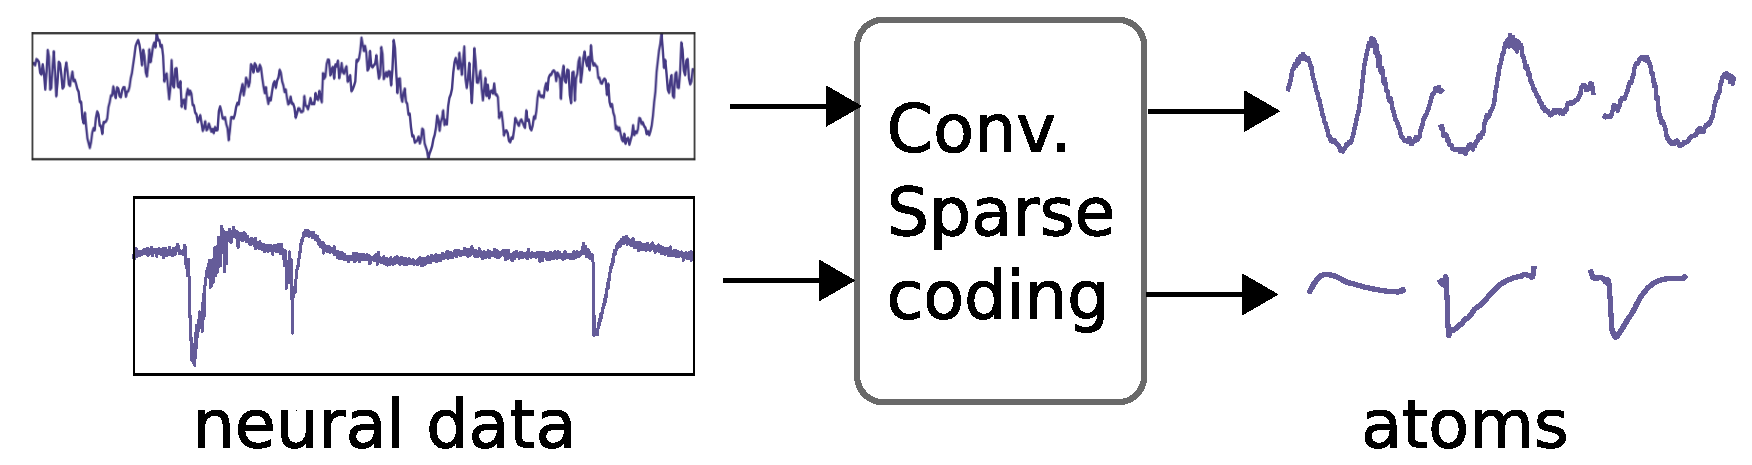
\includegraphics[width=0.7\linewidth]{figures/schema.pdf}
\end{center}
   \caption[Convolutional sparse coding]{An illustration of how Convolutional sparse coding can be used to automatically mine prototypical waveforms}
   \label{fig:neuroimaging_methods}
\end{figure}

However, photos are inherently different from neural data. First, neural data can be buried in noise and corrupted by high amplitude artifacts. Second, images are labelled owing to crowdsourced data as in the case of  Imagenet~\citep{deng2009imagenet}, but neural data is not. 
Expert annotations in the case of neural data are not easily available.
Finally, it is spatiotemporal data with different dynamics than the 3D world that photos capture. This is where \ac{CSC} can play a role by extracting prototypical features from the data. It is an unsupervised algorithm from computer vision, which can learn shift-invariant dictionaries of prototypical waveforms (atoms) from the data using the convolution operations. For a more comprehensive background on \ac{CSC}, the reader may read Section~\ref{sec:background_dict_learning} later in this chapter.

\ac{CSC} algorithms do not approximate the signal using Fourier (or sinusoidal) basis. While this is the conventional technique for extracting signals buried in noise, the approximation can degrade the shape of the signal, which can be a biomarker in many clinical diseases~\citep{cole2017brain}. As an example, a square wave would need an infinite series of sinusoids for a good approximation. Of course, transients can be better approximated using wavelets but it is clearly not sufficient for other shapes of data. Rather than fix the basis to be Fourier or wavelet, the \ac{CSC} approach is to learn \emph{both} the basis and the coefficients.

In our work presented in Chapter~\ref{chapter:alphacsc}, we extend conventional \ac{CSC} algorithms for heavy-tailed noise. We reformulate the optimization problem as a \ac{MAP} inference with an alpha-stable distribution to replace the reconstruction loss. Our results show that this kind of algorithm is robust to the presence of artifacts and can be used to uncover temporal structures from neural signals, even those involving nested oscillations.
